\documentclass[11pt]{article}
\usepackage{amsmath}
\usepackage{pdfpages}
\usepackage{microtype}
\usepackage{algorithm}
\usepackage[noend]{algpseudocode}
\usepackage{setspace}
\usepackage{mathtools}
\DeclarePairedDelimiter\ceil{\lceil}{\rceil}
\DeclarePairedDelimiter\floor{\lfloor}{\rfloor}
\usepackage{hyperref}
\usepackage{listings}
\usepackage{lstautogobble}
\usepackage{float}
\usepackage{amssymb}
\usepackage{physics}
\usepackage[margin=0.75in]{geometry}
\usepackage{multicol}
\usepackage{titlesec}
\usepackage{titling}
\usepackage{graphicx}
\usepackage{xcolor}
\definecolor{codegreen}{rgb}{0,0.6,0}
\definecolor{codegray}{rgb}{0.5,0.5,0.5}
\definecolor{codepurple}{rgb}{0.58,0,0.82}
\definecolor{backcolour}{rgb}{0.95,0.95,0.92}
\lstset{language=C++,
	backgroundcolor=\color{backcolour},   
	commentstyle=\color{codegreen},
	keywordstyle=\color{magenta},
	numberstyle=\tiny\color{codegray},
	stringstyle=\color{codepurple},
	basicstyle=\scriptsize\ttfamily,
	commentstyle=\ttfamily\itshape\color{gray},
	stringstyle=\ttfamily,
	showstringspaces=false,
	breaklines=true,
	autogobble=true
}
\setcounter{tocdepth}{3}
\usepackage[nottoc,notlot,notlof]{tocbibind}
\title{\Huge{ECE470:Network Client-Sever Programming}\\\LARGE{Project 1: Part 1}}
\author{Aaron Jesus Valdes}
\begin{document}
	\maketitle
	\clearpage
	\tableofcontents
	\onehalfspacing
	\clearpage
	\section{Project Description}
	Designing a smart home remote access system which follows the Network/Client architecture. This system allows the user to control certain devices from their home such lights, alarm, and locks from a remote location.
	\section{Project Purpose}
	\section{Project Goals}
	\section{Business Requirement}
		\subsection{Assumptions}
			\begin{itemize}
				\item We are only working with a single house
				\item There are multiple rooms in the house
				\item Each room has multiple lights
				\item There is only one alarm
				\item There are at least 4 locks
				\item One user at a time can connect
				\item The server is in the home
				\item The server can be accessed both inside and outside of the house
				\item The user needs to check and alter status of the devices
				\item The method of communication is
				\item The server must be protected by having a login page
			\end{itemize}
		\subsection{Constraints}
			\begin{itemize}
				\item Does not allow the user to add rooms to the house
				\item Does not allow the user to add lights to the house
				\item Does not allow the user to add locks to the house
				\item Does not allow the user to add new devices to the house
			\end{itemize}
		\subsection{Deliverable}
			\begin{itemize}
				\item Supports smart lights
				\begin{itemize}
					\item Can turn on and off lights
					\item Can turn off all lights for a room
					\item Groups lights into rooms
				\end{itemize}
				\item Supports alarm system
				\begin{itemize}
					\item Can arm and disarm the alarm
					\item Can have more than one alarm system
					\item Can store 4 digit pin per alarm 
					\item Ask the user for a pin to change the alarm
				\end{itemize}
				\item Supports Electronic Locks
				\begin{itemize}
					\item Can open and lock the locks
					\item Can have more than 4 locks
					\item Can store a 5 digit pin per lock
					\item Ask the user for a pin to change the lock
				\end{itemize}
			\end{itemize}
	\section{Design}
		\subsection{Data Model}
			\begin{figure}[H]
				\centering
				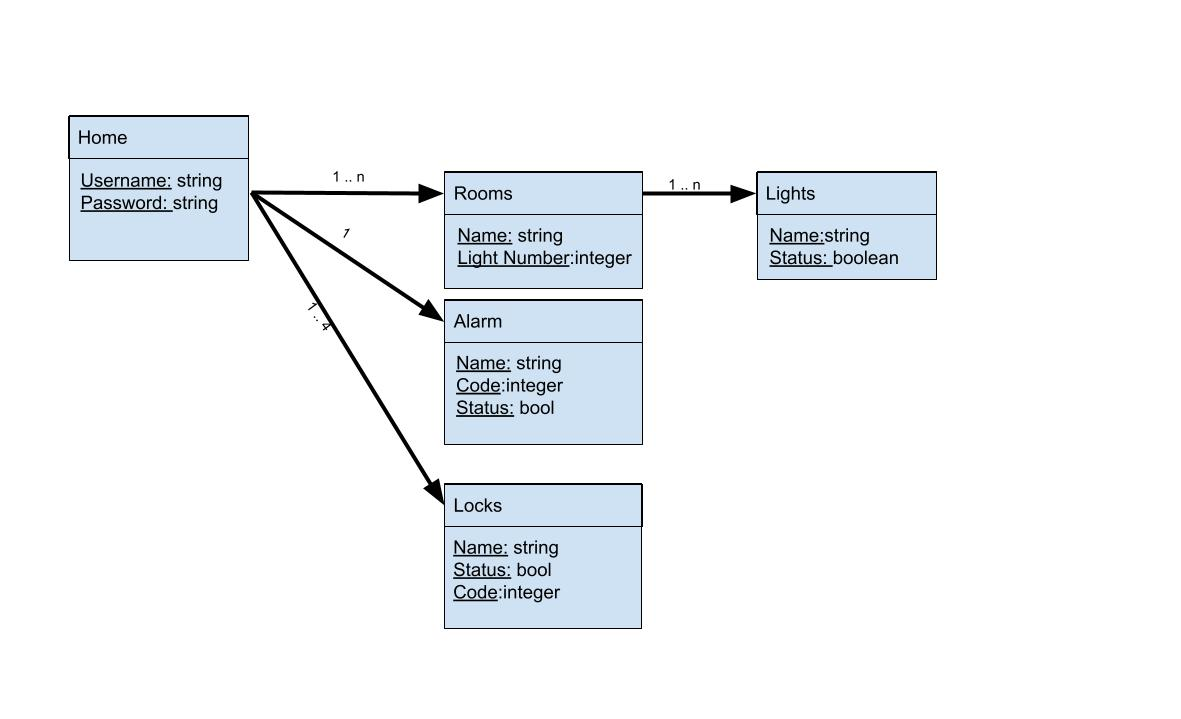
\includegraphics[scale=0.5]{data_model}
				\caption{Data models follow the specifications}
				\label{fig:datamodel}
			\end{figure}
			This is the simplest data model which we can use as a template given the fact that as we move one with this project we are going to be adding more features such as setting RGB colors,change lock combinations, setting the brightness, and later on be able to add more devices
		\subsection{Business Logic}
			\subsubsection{Basic Operations}
				\begin{itemize}
					\item Login/Logout
					\item Check Status of each device
					\item Change Status of each devices
				\end{itemize}
			\subsubsection{Storyboard}
				\begin{figure}[H]
					\centering
					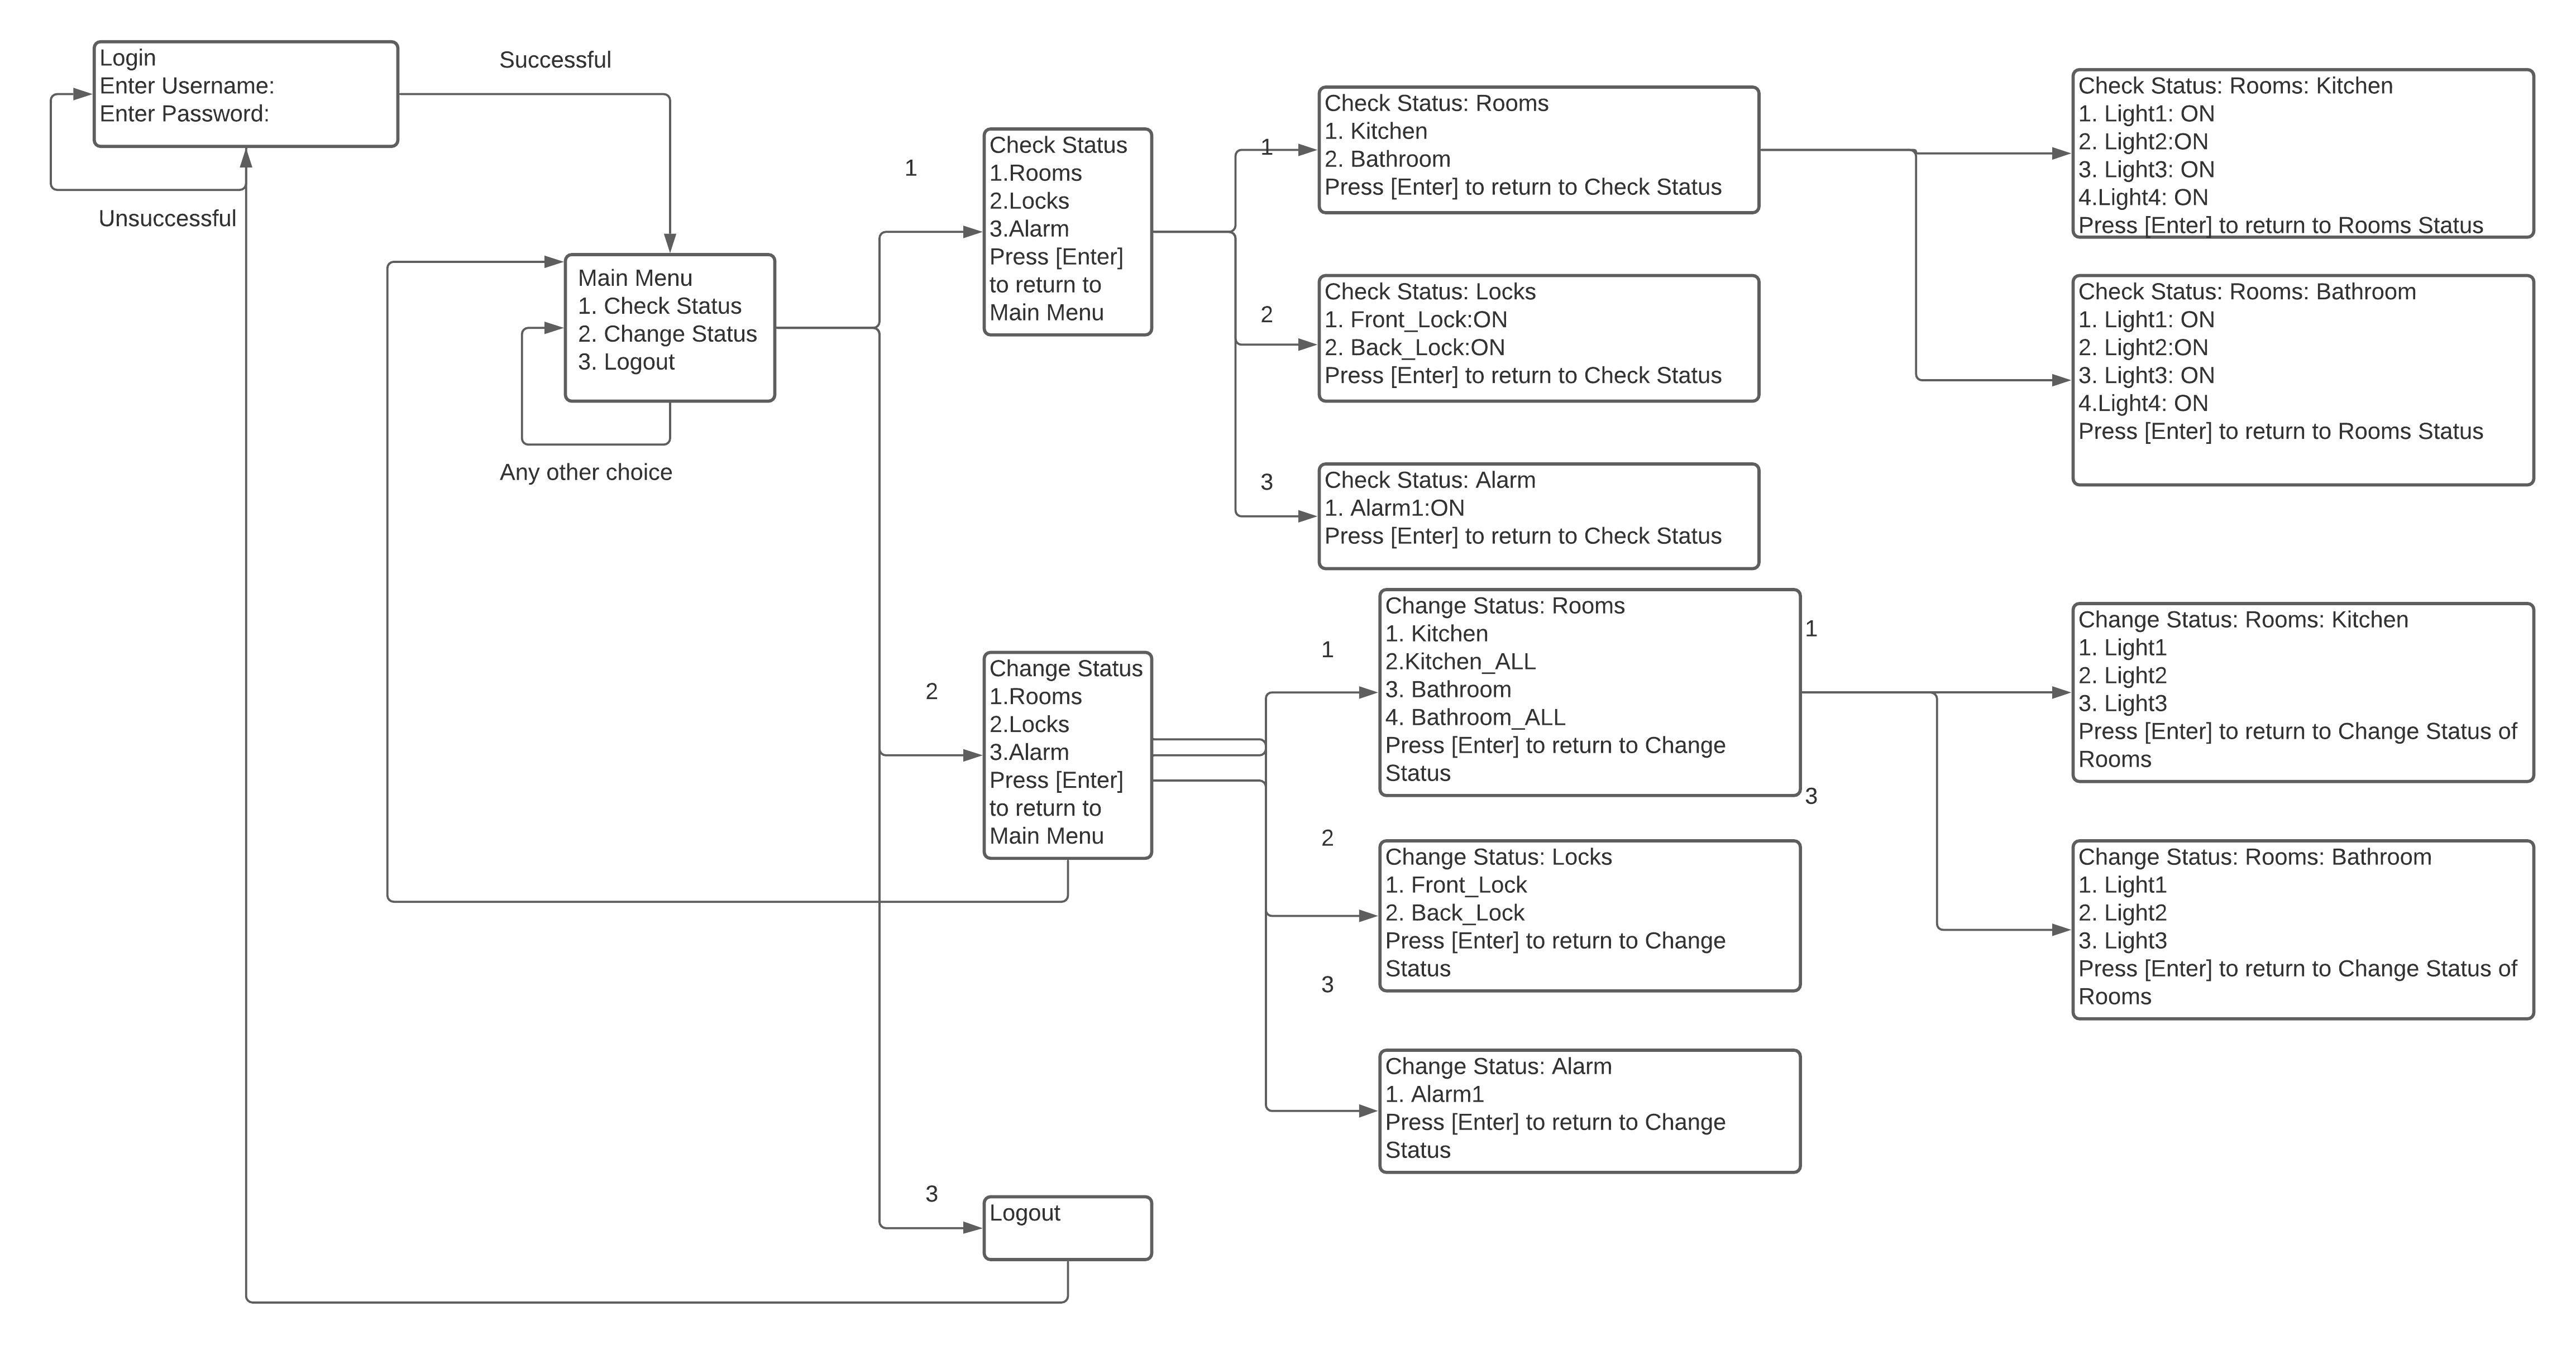
\includegraphics[scale=0.5]{StoryBoard}
					\caption{}
					\label{fig:storyboard}
				\end{figure}
				The reason I chose to divide my check status and change status  based on devices is because that is the method that my google home uses show the status of my devices and change the status of my devices. In my opinion the most effective method is by simply having a single main menu with a all the options since it leads to less amount of packets being transferred back and forth between the client and the server and can therefore reduces bandwidth.
				As we move on, I am going to implement more menus for the alarm,locks, and lights as way to provide more features for each device
			\subsubsection{Sever state chart}
				\begin{figure}[H]
					\centering
					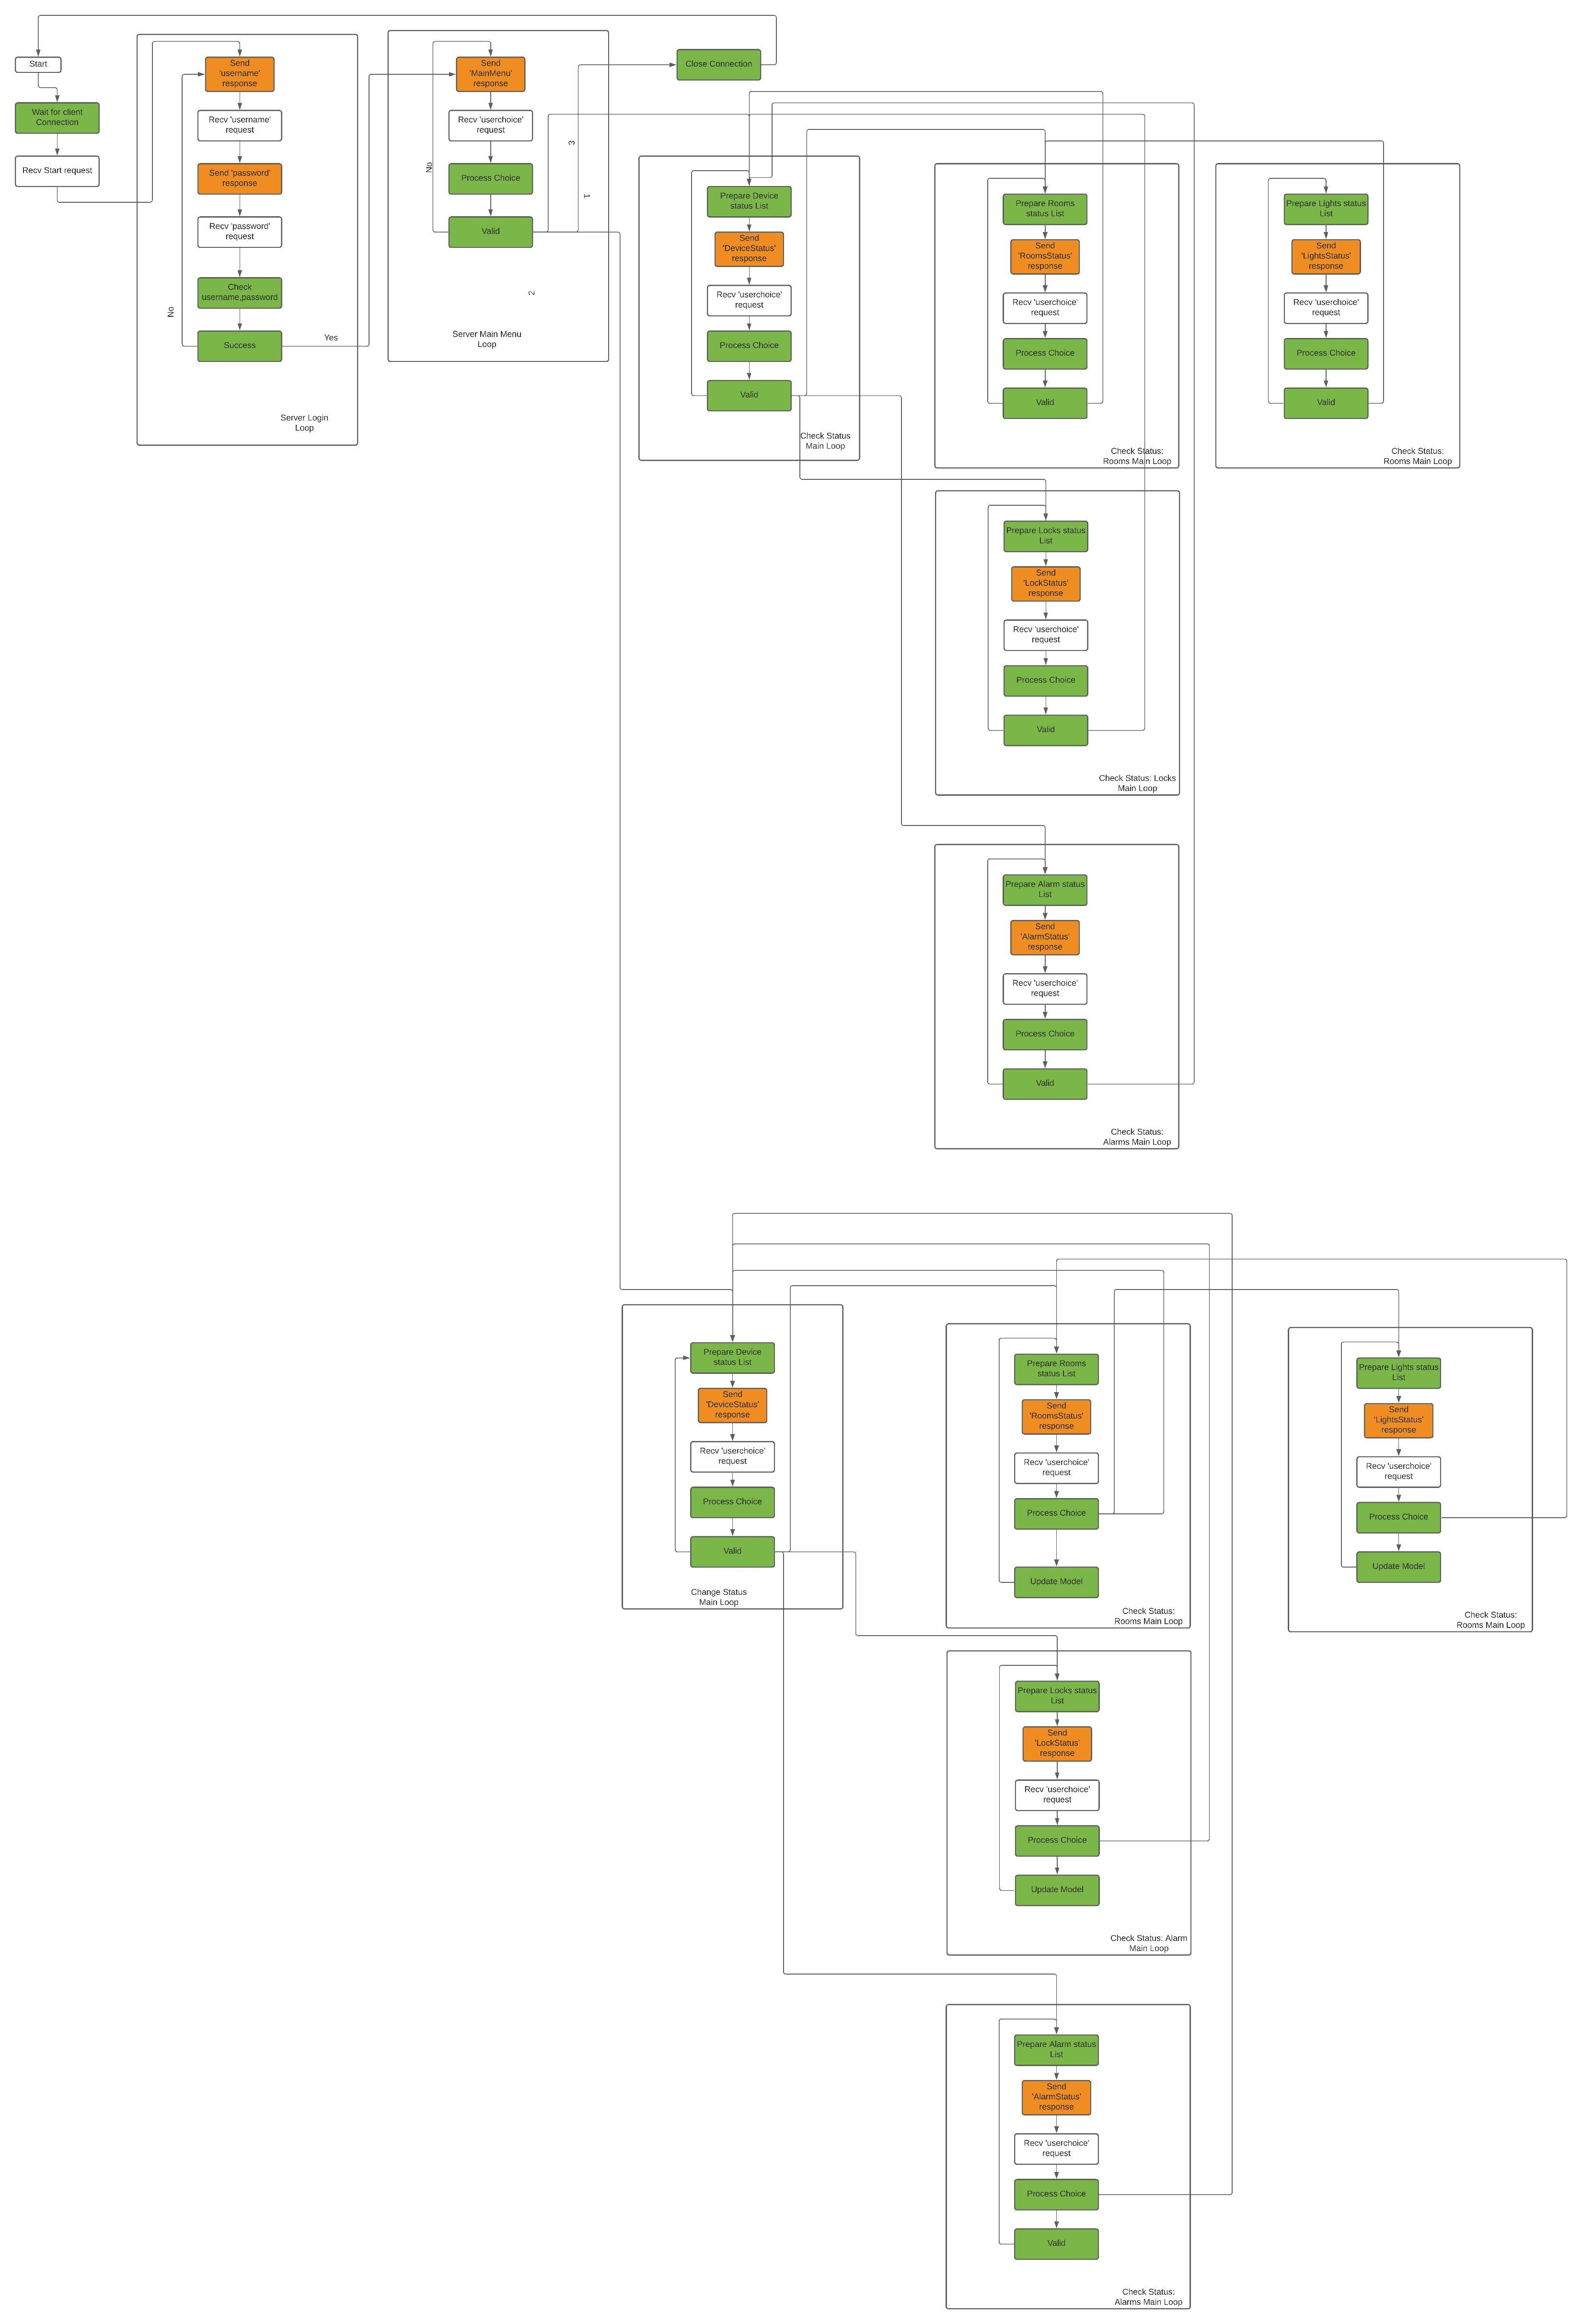
\includegraphics[scale=0.5]{server_state_diagram}
					\label{fig:serverstatediagram}
				\end{figure}
				The server state diagram starts by simply waiting for the client to establish a connection. After establishing a connection, the user is going to be asked to send their username and password which is going to be check by the server based on the data model. If the username and password is correct then we move on to the main menu else we return back to the server login menu. After entering the main menu, the user needs to send the server a request for either checking status of a device, changing the status of a device, or logging out . After the user request the either check or change the status, they are going to receive the list of devices available to choose from. After requesting a device, the user is going to either the rooms, locks, or alarms available to them so they can either change or check the status. For changing the status there is an extra step in which the server updates the data model for each change and returns back to displaying the status of that device. For each menu there is always a return option which is simply by requesting to press enter. 
			\subsubsection{Client State Chart}
				\begin{figure}[H]
					\centering
					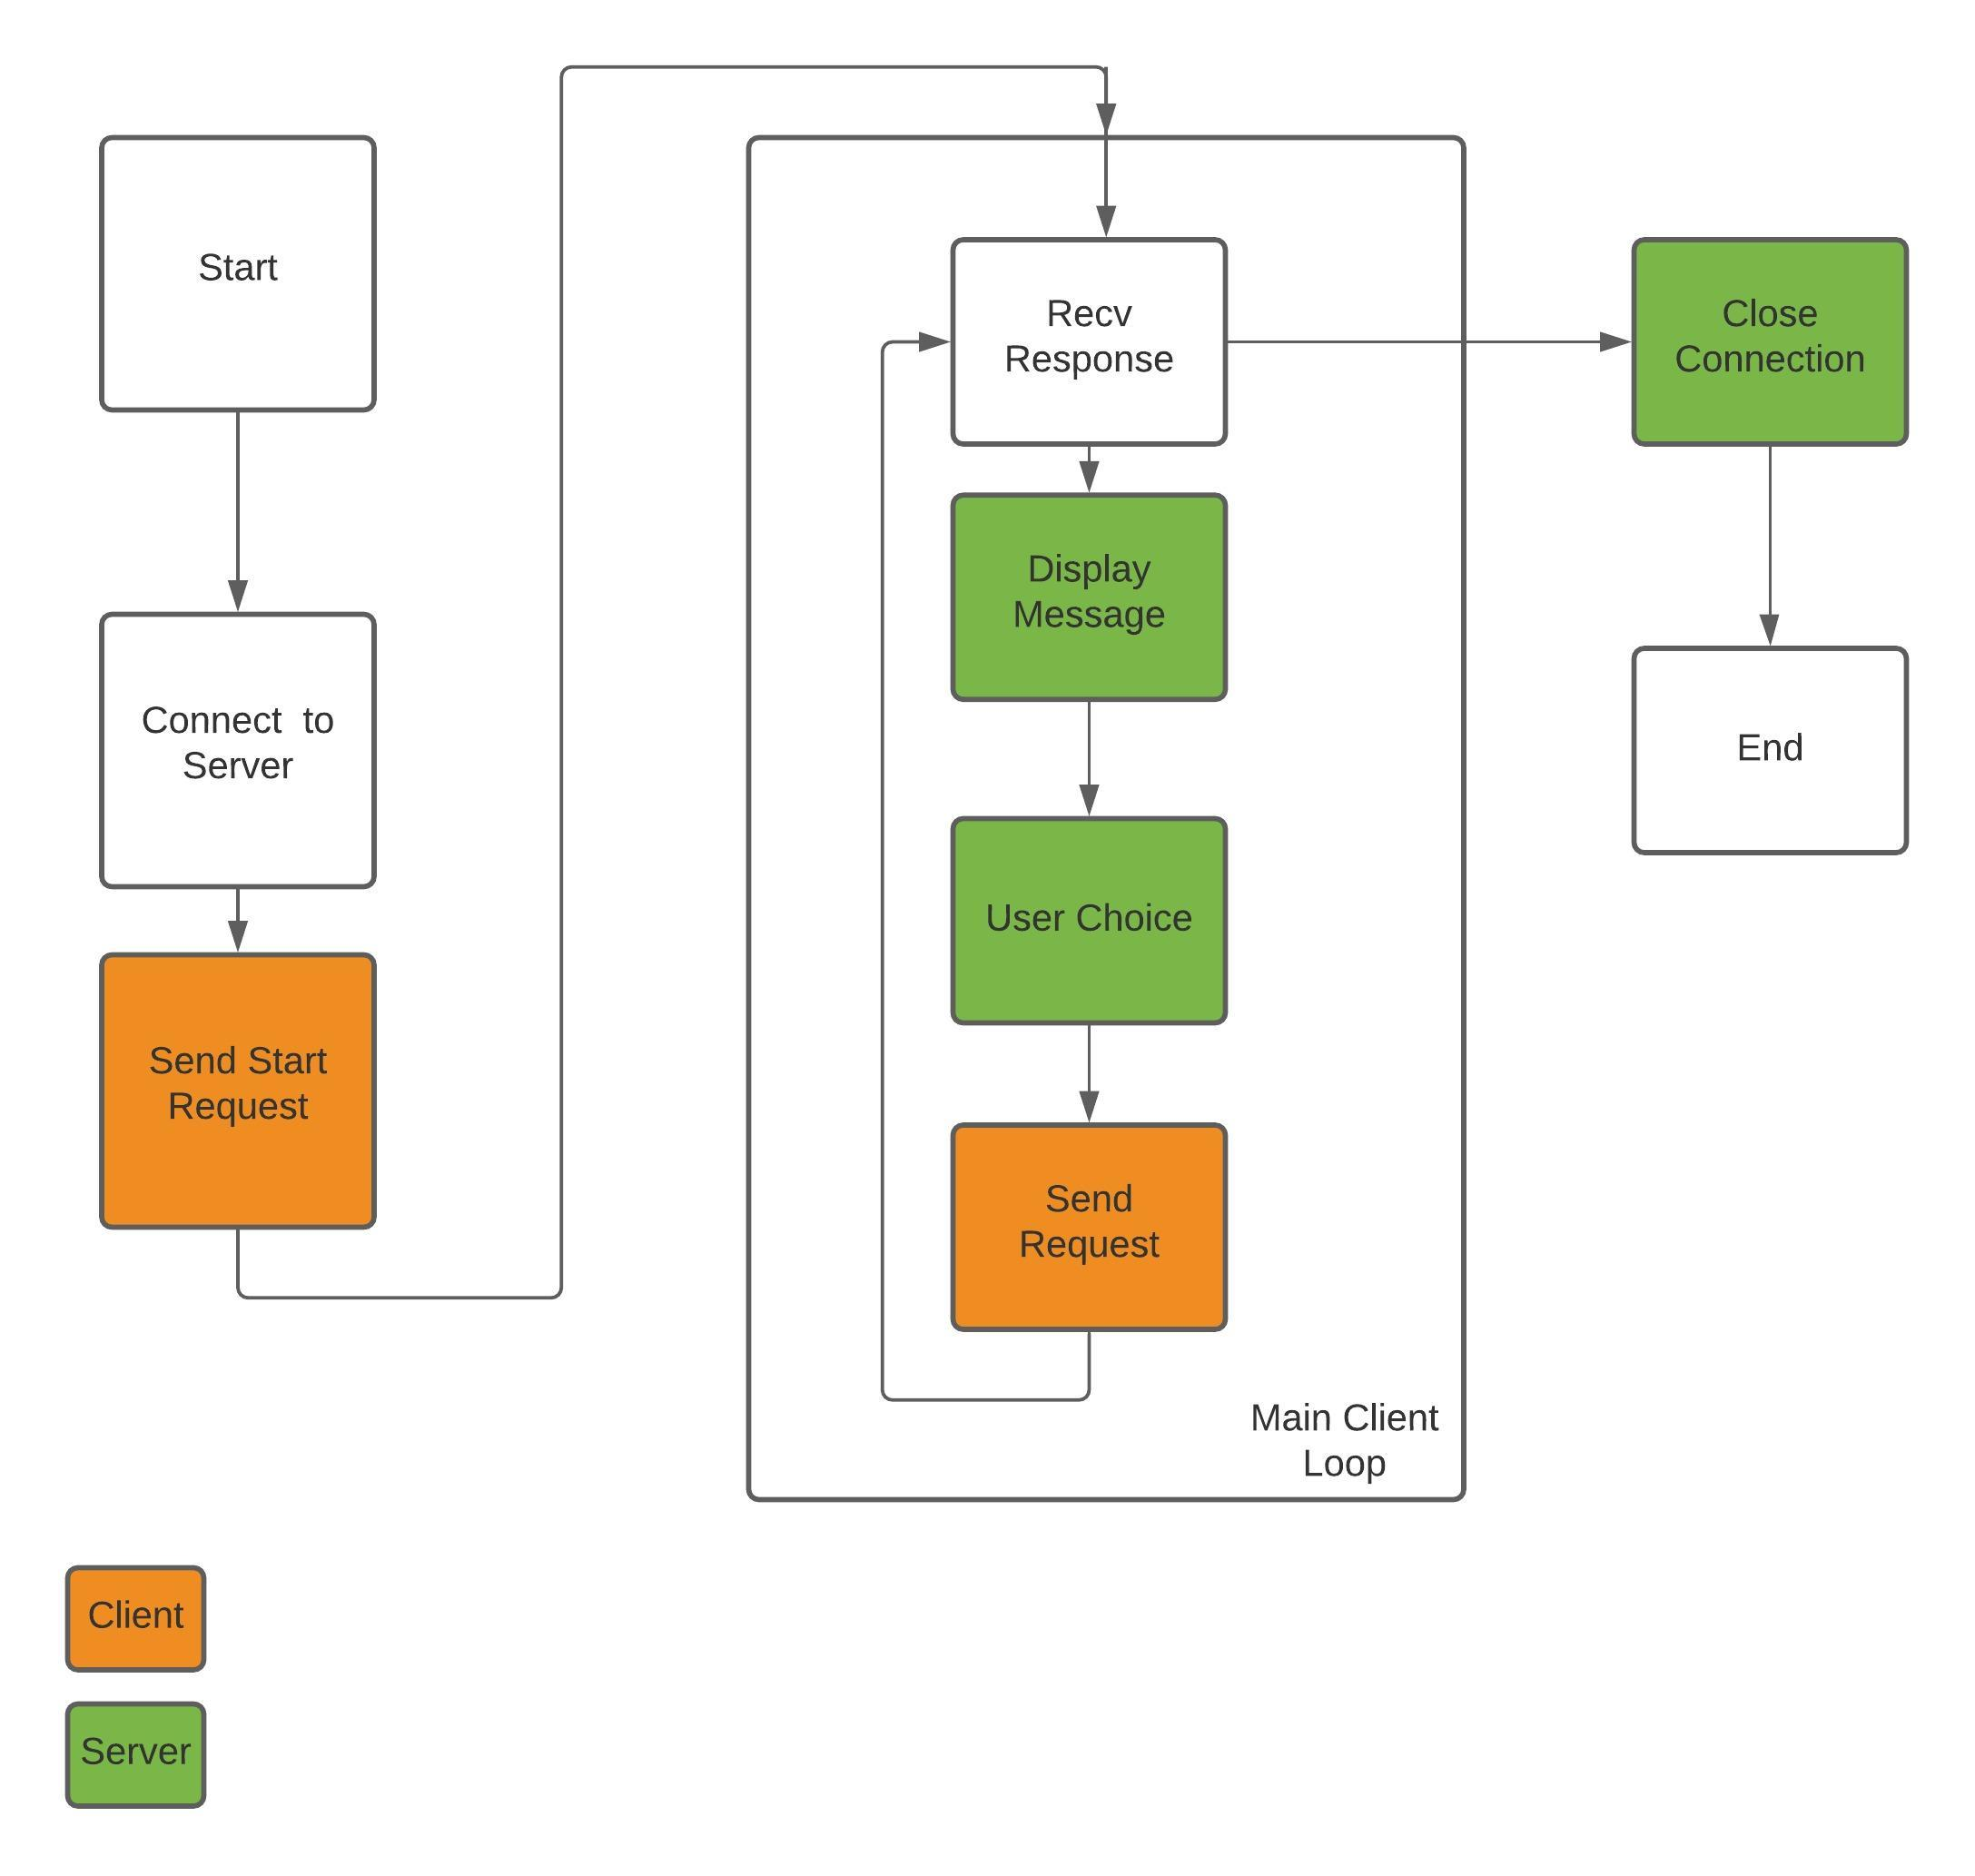
\includegraphics[scale=0.7]{Client_State_Diagram}
					\label{fig:clientstatediagram}
				\end{figure}
				The client state diagram starts by simply establishing a connection between the server and the client. Then the server sends the client a message,which the user uses to make a request. After the request is sent to the server, the server makes a decision based on that request and executes a command. The connection between the server and the client ends when the user decides to log out.
			\subsubsection{Application Protocol Design}
				\begin{table}[H]
					\centering
					\resizebox{\textwidth}{!}{%
						\begin{tabular}{llll}
							\hline
							\multicolumn{1}{|l|}{Client Application Protocols} & \multicolumn{1}{l|}{Parameters}                 & \multicolumn{1}{l|}{Body}    & \multicolumn{1}{l|}{Description}                                                                            \\ \hline
							\multicolumn{1}{|l|}{START}                        & \multicolumn{1}{l|}{none}                       & \multicolumn{1}{l|}{none}    & \multicolumn{1}{l|}{Establishes connection with the server}                                                 \\ \hline
							\multicolumn{1}{|l|}{CHOICE}                       & \multicolumn{1}{l|}{Lines=24 character,lines=0} & \multicolumn{1}{l|}{None}    & \multicolumn{1}{l|}{Based on the options of the server, the user can send up to 24 character to the server} \\ \hline
							\multicolumn{1}{|l|}{END}                          & \multicolumn{1}{l|}{None}                       & \multicolumn{1}{l|}{none}    & \multicolumn{1}{l|}{Ends the connection between the client and the server}                                  \\ \hline
							&                                                 &                              &                                                                                                             \\
							&                                                 &                              &                                                                                                             \\
							&                                                 &                              &                                                                                                             \\ \hline
							\multicolumn{1}{|l|}{Server Application Protocols} & \multicolumn{1}{l|}{Parameters}                 & \multicolumn{1}{l|}{Body}    & \multicolumn{1}{l|}{Description}                                                                            \\ \hline
							\multicolumn{1}{|l|}{USER}                         & \multicolumn{1}{l|}{Lines=24 character}         & \multicolumn{1}{l|}{Line}    & \multicolumn{1}{l|}{Ask the user for the username}                                                          \\ \hline
							\multicolumn{1}{|l|}{PASS}                         & \multicolumn{1}{l|}{Line=24 character}          & \multicolumn{1}{l|}{Line}    & \multicolumn{1}{l|}{Ask the user for the password}                                                          \\ \hline
							\multicolumn{1}{|l|}{LIST}                         & \multicolumn{1}{l|}{Line=24 character}          & \multicolumn{1}{l|}{Line(s)} & \multicolumn{1}{l|}{Gives the user options which they can chose from}                                       \\ \hline
							\multicolumn{1}{|l|}{ERROR}                        & \multicolumn{1}{l|}{Line=24 character}          & \multicolumn{1}{l|}{Line(s)} & \multicolumn{1}{l|}{Send the user information about an error in the system and waits for his choice}        \\ \hline
							\multicolumn{1}{|l|}{END}                          & \multicolumn{1}{l|}{None}                       & \multicolumn{1}{l|}{None}    & \multicolumn{1}{l|}{The server ends the connection between the client and the server}                       \\ \hline
						\end{tabular}
					}
				\end{table}
			\subsubsection{Example}
				\begin{figure}[H]
					\centering
					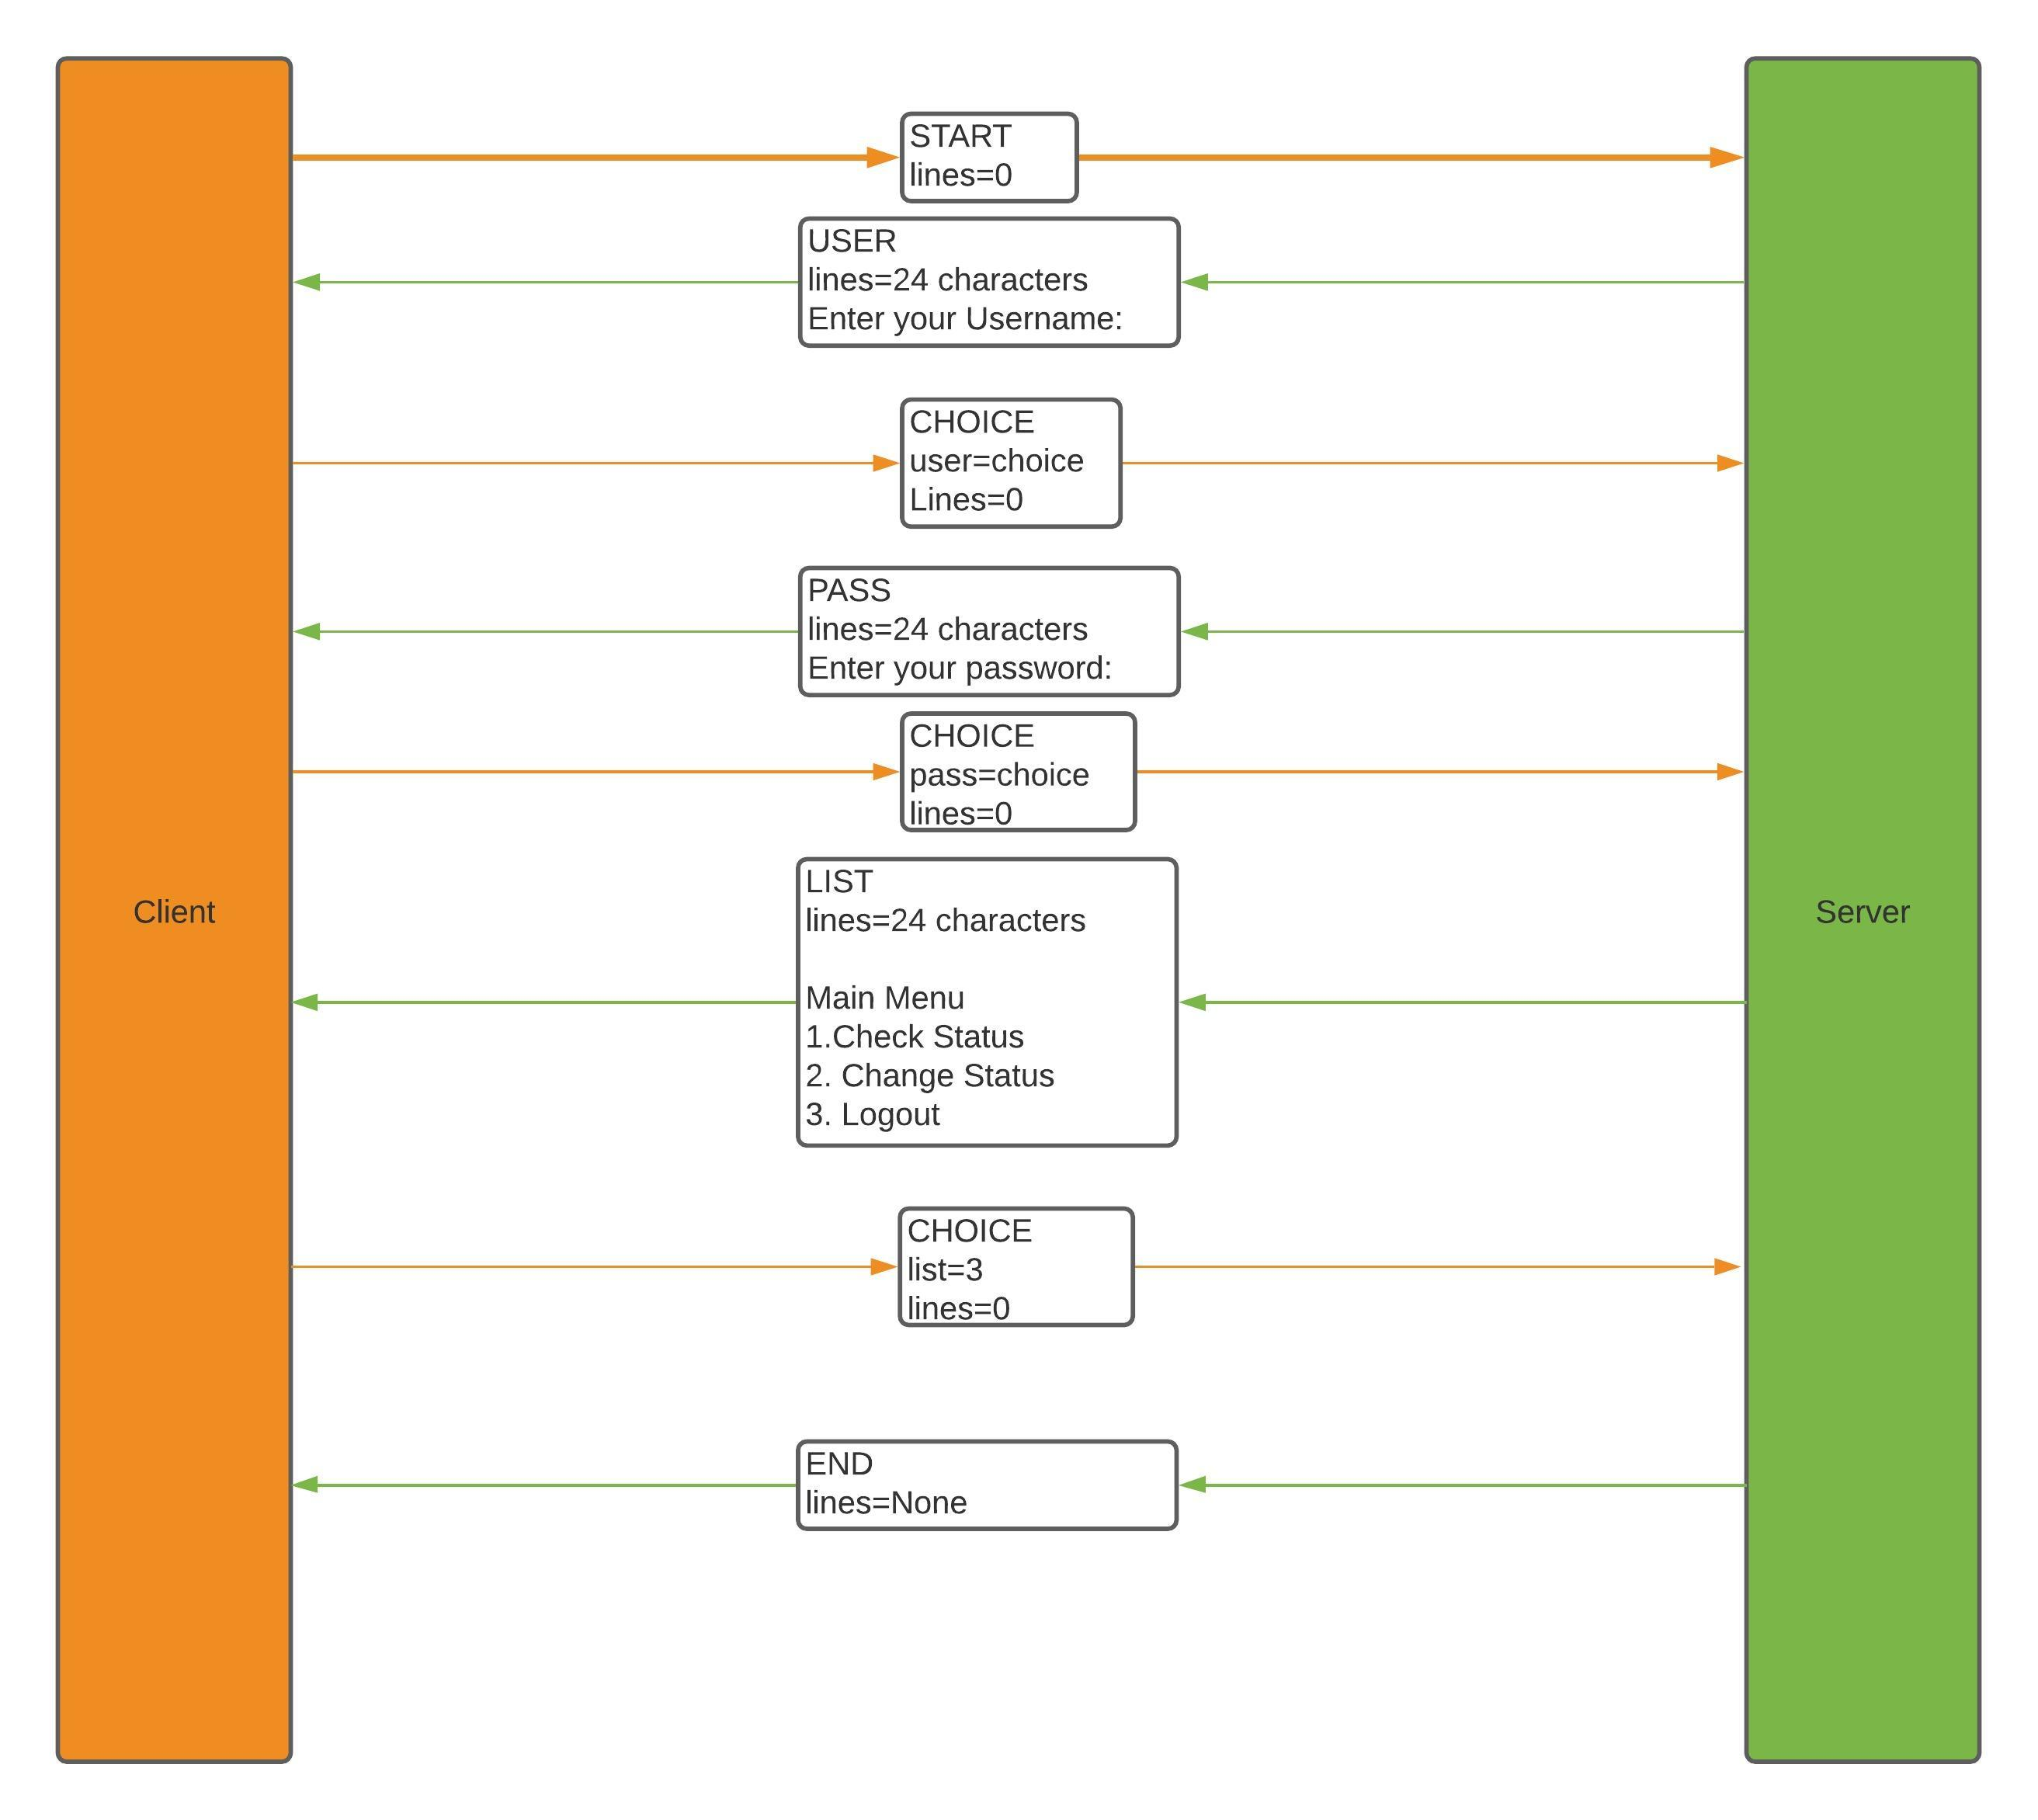
\includegraphics[scale=0.7]{Examples}
					\label{fig:examples}
				\end{figure}
	\section{Implementation}
		My steps for the implementation
		\begin{enumerate}
			\item Create the client marshal and test that it works
			\item Create the server marshal and test that it works
			\item Create the network for the client to send and receive
			\item Create the network for the server to send and receive
			\item Create the main for the client
				\subitem Follow the business model for the client
				\subitem Make sure that it is able to send and receive
			\item Create the login menu for the server
			\item Create the main menu for the server
			\item Create the check status menu
			\item Create the change status menu
			\item Create the the an alarm menu
				\subitem With the option to create a specific menu for check and change status
				\subitem For change alarm status ask the user for a pin to be able to change the status
			\item Create the rooms menu
			\item Create the lights menu
				\subitem With the option to create a specific menu for check and change status and for the individual room
				\subitem Add the option to either change all lights or a single light
			\item Create the locks menu
				\subitem With the option to create a specific menu for check and change status
				\subitem For change lock status ask the user for a pin to be able to change the status of either all locks or individual locks
		\end{enumerate}
	\section{Testing}
	\begin{figure}[H]
		\centering
		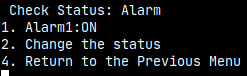
\includegraphics[scale=0.7]{testing_change_alarmStatus}
		\caption[Testing Changing Alarm Status]{}
		\label{fig:testingchangealarmstatus}
	\end{figure}
	\begin{figure}[H]
		\centering
		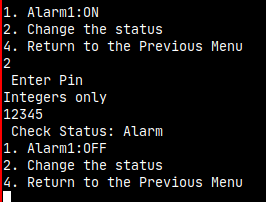
\includegraphics[scale=0.7]{testing_changealarmstatus_pin}
		\caption[Testing changing alarm status with the pin]{}
		\label{fig:testingchangealarmstatuspin}
	\end{figure}
	\begin{figure}[H]
		\centering
		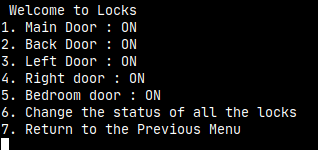
\includegraphics[scale=0.7]{testing_change_locksstatus}
		\caption[Testing change lock status]{}
		\label{fig:testingchangelocksstatus}
	\end{figure}
	\begin{figure}[H]
		\centering
		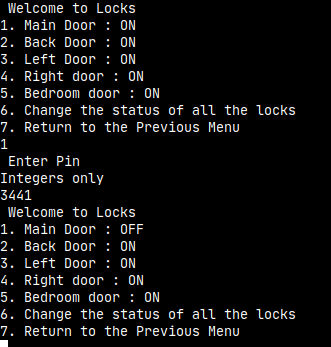
\includegraphics[scale=0.7]{testing_change_locksstatus_pin}
		\caption[Testing change lock status with pin]{}
		\label{fig:testingchangelocksstatuspin}
	\end{figure}
	\begin{figure}[H]
		\centering
		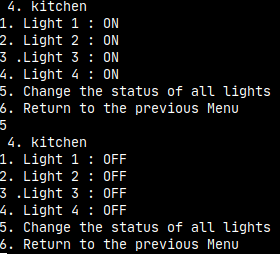
\includegraphics[scale=0.7]{testing_changestatus_allights}
		\caption[Testing change status of all lights]{}
		\label{fig:testingchangestatusallights}
	\end{figure}
	\begin{figure}[H]
		\centering
		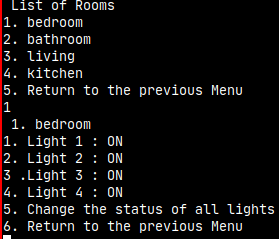
\includegraphics[scale=0.7]{testing_change_status_lights}
		\caption[Testing change status of a single light]{}
		\label{fig:testingchangestatuslights}
	\end{figure}
	\begin{figure}[H]
		\centering
		\includegraphics[scale=0.7]{"testing_changestatus_single light"}
		\caption[Testing change status of a single light]{}
		\label{fig:testingchangestatussingle-light}
	\end{figure}
	\begin{figure}[H]
		\centering
		\includegraphics[scale=0.7]{"testing_check alarm"}
		\caption[Testing checking the alarm]{}
		\label{fig:testingcheck-alarm}
	\end{figure}
	\begin{figure}[H]
		\centering
		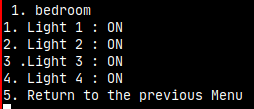
\includegraphics[scale=0.7]{testing_checkbedroom_lights}
		\caption[Testing check the bedroom lights]{}
		\label{fig:testingcheckbedroomlights}
	\end{figure}
	\begin{figure}[H]
		\centering
		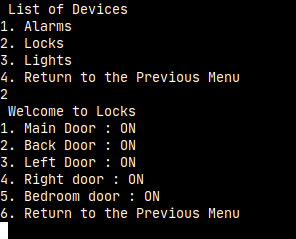
\includegraphics[scale=0.7]{testing_checklock}
		\caption[Testing check the lock status]{}
		\label{fig:testingchecklock}
	\end{figure}
	\begin{figure}[H]
		\centering
		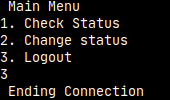
\includegraphics[scale=0.7]{testing_ending_connection}
		\caption[Testing ending connection]{}
		\label{fig:testingendingconnection}
	\end{figure}
	\begin{figure}[H]
		\centering
		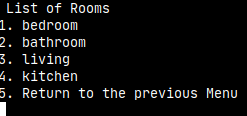
\includegraphics[scale=0.7]{testing_lightRoom}
		\caption[Testing check status of lights in a room]{}
		\label{fig:testinglightroom}
	\end{figure}
	\begin{figure}[H]
		\centering
		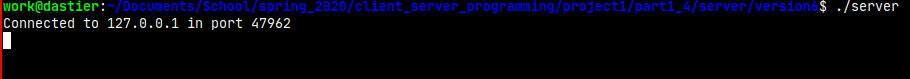
\includegraphics[scale=0.5]{testing_serverconnection}
		\caption[Testing server connection]{}
		\label{fig:testingserverconnection}
	\end{figure}
	\begin{figure}[H]
		\centering
		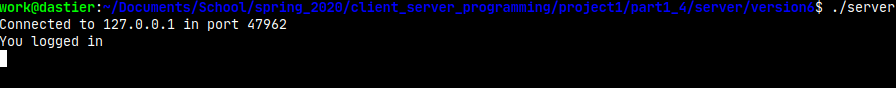
\includegraphics[scale=0.5]{testing_serverlogin}
		\caption[Testing server login]{}
		\label{fig:testingserverlogin}
	\end{figure}
	\begin{figure}[H]
		\centering
		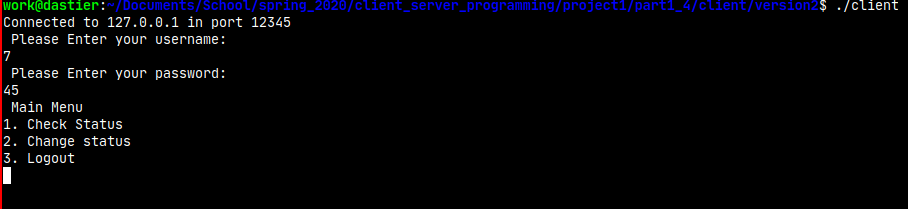
\includegraphics[scale=0.5]{testing_Succesful_login}
		\caption[Testing succesfull login]{}
		\label{fig:testingsuccesfullogin}
	\end{figure}
	\begin{figure}[H]
		\centering
		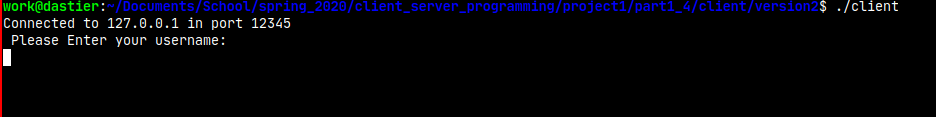
\includegraphics[scale=0.5]{testing_userName}
		\caption[Testing username menu]{}
		\label{fig:testingusername}
	\end{figure}
	\section{Conclusion}
		Overall this project took a lot of time, which I didn't expect it would take since I though the implementation was going to be easy. Either way I was able to implement a working program that can handle the simplest features and can easily expand to others such having smart lights which can be dimmed or change the color. Furthermore, this program can be further improve by having a hashing function for the password and username since that can help us with the security aspect of it. Furthermore we can add more features to make sure that the user does not put anything that is not an integer as a choice.
	\section{Appendix-Code}
		\subsection{Data model}
			\begin{lstlisting}[language=C++]
				#ifndef _DATAMODEL_H_
				#define _DATAMODEL_H_
				#include <iostream>
				#include <string>
				#include <vector>
				#include <sstream>
				using namespace std;
				
				
				class light
				{
				public:
				string name;
				bool status;
				light();
				light(string name,bool status);
				};
				
				light::light()
				{
				name="Bedroom Light";
				status=true;
				}
				light::light(string name1, bool status1)
				{
				name=name1;
				status=status1;
				}
				
				
				class room
				{
				public:
				vector<light> lights;
				vector<string> lightsList;
				string roomName;
				int roomNumber;
				int numLights;
				room();
				room(string roomMa ,int ro);
				void setLightList();
				void changeAllLights();
				void changeSingleLights(int option);
				};
				
				void room::changeAllLights()
				{
				for(unsigned int i=0;i<lights.size();i++)
				{
				lights[i].status=!lights[i].status;
				}
				setLightList();
				}
				
				void room::changeSingleLights(int option)
				{
				lights[option].status=!lights[option].status;
				setLightList();
				}
				
				void room::setLightList()
				{
				vector<string> tempLight;
				for(unsigned int i=0;i<lights.size();i++)
				{
				stringstream ss;
				string lightSta;
				string temp;
				if(lights[i].status)
				{
				lightSta="ON";
				}
				else
				{
				lightSta="OFF";
				}
				ss<<lights[i].name<<" : "<<lightSta;
				getline(ss,temp);
				tempLight.push_back(temp);
				}
				lightsList=tempLight;
				}
				
				
				room::room()
				{
				light t1("Light 1",true);
				light t2("Light 2",true);
				light t3("Light 3",true);
				light t4("Light 4",true);
				lights.push_back(t1);
				lights.push_back(t2);
				lights.push_back(t3);
				lights.push_back(t4);
				roomName="Bedroom";
				numLights=lights.size();
				roomNumber=1;
				setLightList();
				}
				
				room::room(string roomNa,int ro)
				{
				roomNumber=ro;
				stringstream ss;
				string temp;
				ss<<roomNumber<<". "<<roomNa;
				getline(ss,temp);
				light t1("1. Light 1",true);
				light t2("2. Light 2",true);
				light t3("3 .Light 3",true);
				light t4("4. Light 4",true);
				lights.push_back(t1);
				lights.push_back(t2);
				lights.push_back(t3);
				lights.push_back(t4);
				roomName=temp;
				numLights=lights.size();
				setLightList();
				}
				
				
				
				class rooms
				{
				private:
				public:
				vector<room> house_room;
				int numRoom;
				rooms();
				vector<string> roomList;
				int obtainNumberofRooms()
				{
				return numRoom;
				}
				void setRoomList();
				};
				
				rooms::rooms()
				{
				room bedroom("bedroom",1);
				room bathroom("bathroom",2);
				room livingroom("living",3);
				room kitchen("kitchen",4);
				house_room.push_back(bedroom);
				house_room.push_back(bathroom);
				house_room.push_back(livingroom);
				house_room.push_back(kitchen);
				numRoom=house_room.size();
				setRoomList();
				}
				
				void rooms::setRoomList()
				{
				for(unsigned int i=0;i<house_room.size();i++)
				{
				roomList.push_back(house_room[i].roomName);
				}
				}
				
				
				class alarmSystem
				{
				private:
				bool status;
				int code;
				public:
				alarmSystem()
				{
				status=true;
				code=12345;
				};
				string name; 
				
				void changeStatus(int opt)
				{
				if(opt==code)
				{
				status=!status;
				}
				}
				
				bool getStatus()
				{
				return status;
				};
				};
				
				
				
				class lock
				{
				public:
				string name;
				int code;
				bool status;
				lock();
				lock(string nam,bool stat,int codd); 
				};
				
				lock::lock()
				{
				name="Main";
				code=12345;
				status=true;
				}
				
				lock::lock(string nam,bool stat,int codd)
				{
				name=nam;
				code=codd;
				status=stat;
				}
				
				class locks
				{
				private:
				int masterLock;
				public:
				vector<lock> llock;
				vector <string> locksList;
				int numLocks;
				locks();
				void setLocksList();
				void changeAllLocks(int opt);
				void changeSingleLock(int option, int opt);
				};
				
				void locks::changeAllLocks(int opt)
				{
				if(opt==masterLock)
				{
				for(unsigned int i=0;i<llock.size();i++)
				{
				llock[i].status=!llock[i].status;
				}
				setLocksList();
				}
				}
				
				void locks::changeSingleLock(int option,int opt)
				{
				if(opt==llock[option].code)
				{
				llock[option].status=!llock[option].status;
				setLocksList();
				}
				}
				
				locks::locks()
				{
				lock ll1("1. Main Door",true,3441);
				lock ll2("2. Back Door",true,1234);
				lock ll3("3. Left Door",true,7812);
				lock ll4("4. Right door",true,2232);
				lock ll5("5. Bedroom door",true,2131);
				llock.push_back(ll1);
				llock.push_back(ll2);
				llock.push_back(ll3);
				llock.push_back(ll4);
				llock.push_back(ll5);
				numLocks=llock.size();
				setLocksList();
				}
				
				void locks::setLocksList()
				{
				vector<string> tempLock;
				for(unsigned int i=0;i<llock.size();i++)
				{
				stringstream ss;
				string lightSta;
				string temp;
				if(llock[i].status)
				{
				lightSta="ON";
				}
				else
				{
				lightSta="OFF";
				}
				ss<<llock[i].name<<" : "<<lightSta;
				getline(ss,temp);
				tempLock.push_back(temp);
				}
				locksList=tempLock;
				}
				
				class home
				{
				private:
				string password;
				string username;
				public:
				vector<string> deviceList;
				rooms ro;
				alarmSystem al;
				locks lo;
				home(); 
				void setDeviceList();
				};
				
				
				void home::setDeviceList()
				{
				deviceList.push_back("1. Alarms");
				deviceList.push_back("2. Locks");
				deviceList.push_back("3. Lights");
				}
				
				home::home()
				{
				setDeviceList();
				}
				#endif
			\end{lstlisting}
		\subsection{Message Protocol}
		\subsection{Client Marshal}
			\subsubsection{Header file}
				\begin{lstlisting}[language=C++]
					#ifndef _CLIENT_MARSHAL_H_
					#define _CLIENT_MARSHAL_H_
					#include <iostream>
					#include <string>
					#include <stdio.h>
					#include <stdlib.h>
					#include <sstream>
					#include <vector>
					using namespace std;
					class server_message
					{
					public:
					string options;
					string message;
					vector<string> lines;
					int num_lines;
					void printingDebug()
					{
					cout<<options<<"    "<<num_lines<<"     "<<message<<endl;
					for(unsigned int i=0;i<lines.size();i++)
					{
					cout<<lines[i]<<endl;
					}
					
					}
					void printing()
					{
					cout<<message<<endl;
					for(unsigned int i=0;i<lines.size();i++)
					{
					cout<<lines[i]<<endl;
					}
					
					}
					};
					
					class client_message
					{
					public:
					string options;
					int decision;
					void printing()
					{
					cout<<options<<"    "<<decision;
					}
					};
					
					server_message unmarshal(string message)
					{
					string command;
					server_message res;
					stringstream ss(message);
					ss>>command;
					if(command=="USER")
					{   res.options="USER";
					getline(ss,res.message);
					}
					else if(command=="PASS")
					{
					res.options="PASS";
					getline(ss,res.message);
					}
					else if(command=="LIST")
					{
					res.options="LIST";
					getline(ss,res.message,'\\');
					ss>>res.num_lines;
					vector<stringstream> tt(res.num_lines);
					string temp;
					int i=0;
					while(ss>>temp)
					{
					if(temp=="\\")
					{
					i++;
					}
					else
					{
					tt[i]<<temp<<" ";
					}
					}
					for(unsigned int j=0;j<tt.size();j++)
					{
					string temp2;
					getline(tt[j],temp2);
					res.lines.push_back(temp2);
					}
					}
					else if(command=="ERROR")
					{
					res.options="ERROR";
					getline(ss,res.message);
					ss>>res.message;
					}
					else if(command=="END")
					{
					res.options="END";
					getline(ss,res.message);
					ss>>res.message;
					}
					else
					{
					}
					return res;
					}
					
					
					string marshal(client_message cm)
					{
					stringstream ss;
					string result;
					if(cm.options=="START")
					{
					ss<<cm.options<<" "<<cm.decision;
					}
					else if(cm.options=="CHOICE")
					{
					ss<<cm.options<<" "<<cm.decision;
					}
					else if(cm.options=="END")
					{
					ss<<cm.options<<" "<<cm.decision;
					}
					else if(cm.options=="ERROR")
					{
					ss<<cm.options<<" "<<cm.decision;
					}
					else
					{
					} 
					getline(ss,result);
					return result;
					}
					
					
					#endif
				\end{lstlisting}
			\subsubsection{Test File}
				\begin{lstlisting}[language=C++]
					#include <iostream>
					#include <string>
					#include <stdio.h>
					#include <stdlib.h>
					#include <sstream>
					#include "client_marshal.h"
					using namespace std;
					int main(int argc,char*argv[])
					{
					if(argc==2)
					{
					cout<<"Testing unmarshal"<<endl;
					server_message test1;
					test1 =unmarshal(argv[1]);
					test1.printing();
					}
					
					if(argc>2)
					{
					cout<<"Testing Marshall"<<endl;
					client_message test;
					test.decision=atoi(argv[2]);
					test.options=argv[1];
					cout<<marshal(test)<<endl;
					}
					return 0;
					}
				\end{lstlisting}
			\subsubsection{Makefile}
				\begin{lstlisting}[language=C++]
					all:client server_marshal.h client_marshal.h
					echo Testing the client
					client:client.cpp client_marshal.h
					g++ client.cpp -o client				
					test_client: client client.cpp client_marshal.h
					@./client "USER Enter Your Username:"
					@./client "PASS Enter your Password:"
					@./client "ERROR There is an Error:"
					@./client "END Ending the Connection"
					@./client "LIST Here are the options: \ 1 1.Option 1 \\"
					@./client "LIST Here are the options: \ 2 1.Option 1 \ 2. Option 2 \\"
					@./client "LIST Here are the options: \ 3 1.Option 1 \ 2. Option 2 \ 3. Option 3 \\"
					@./client "LIST Here are the options: \ 4 1.Option 1 \ 2. Option 2 \ 3. Option 3 \ 4. Option 4 \\"
					@ echo
					@ echo
					@./client "START" "1"
					@./client "CHOICE" "1"
					@./client "END" "1"
					@./client "ERROR" "1"
					clean:
					rm client
				\end{lstlisting}
			\subsection{Results}	
					\begin{figure}[H]
						\centering
						\includegraphics[scale=0.7]{"../../../../../../../Pictures/Screenshot from 2021-03-02 21-02-45"}
						\caption{Results for the client marshalling}
						\label{fig:screenshot-from-2021-03-02-21-02-45}
					\end{figure}
		\subsection{Server Marshal}
				\subsubsection{Header File}
					\begin{lstlisting}[language=C++]
						#ifndef _SERVER_MARSHAL_H_
						#define _SERVER_MARSHAL_H_
						#include <iostream>
						#include <string>
						#include <stdio.h>
						#include <stdlib.h>
						#include <sstream>
						#include <vector>
						using namespace std;
						
						class client_message
						{
						public:
						string command;
						int decision;
						void printing()
						{
						cout<<command<<"    "<<decision<<endl;
						}
						};
						
						class server_message
						{
						public:
						string command;
						string messa;
						vector<string> lines;
						int num_lines;
						};
						
						struct samples_serverMessage
						{
						server_message userNameResponse;
						server_message passWordResponse;
						server_message create_userNameResponse()
						{
						userNameResponse.command="USER";
						userNameResponse.messa="Please Enter your username:";
						return userNameResponse;
						};
						
						server_message create_passWordResponse()
						{
						passWordResponse.command="PASS";
						passWordResponse.messa="Please Enter your password:";
						return passWordResponse;
						};
						};
						
						
						client_message unmarshal(string message)
						{
						string command;
						int decision;
						client_message res;
						istringstream ss(message);
						ss>>command>>decision;
						res.command=command;
						res.decision=decision;
						return res;
						}
						
						string marshal(server_message sm)
						{
						stringstream ss;
						string result;
						string c[5]={"USER","PASS","LIST","ERROR","END"};
						if(sm.command == c[0])
						{
						ss<<sm.command<<" "<<sm.messa<<" ";
						}
						else if(sm.command == c[1])
						{
						ss<<sm.command<<" "<<sm.messa<<" ";
						}
						else if(sm.command == c[2])
						{
						ss<<sm.command<<" "<<sm.messa<<" "<<"\\"<<" "<<sm.num_lines;
						for(int i=0;i<sm.num_lines;i++)
						{
						ss<<" "<<sm.lines[i]<<" "<<"\\";
						}
						}
						else if(sm.command == c[3])
						{
						ss<<sm.command<<" "<<sm.messa;
						}
						else if(sm.command == c[4])
						{
						ss<<sm.command<<" "<<sm.messa;
						}
						else
						{
						}
						getline(ss,result);
						return result;
						}
						#endif
					\end{lstlisting}
				\subsubsection{Test program}
					\begin{lstlisting}[language=C++]
						#include "server_marshal.h"
						using namespace std;
						
						int main(int argc,char*argv[])
						{
						if(argc<3)
						{
						cout<<"Testing unmarshal"<<endl;
						client_message test=unmarshal(argv[1]);
						test.printing();
						}
						else
						{
						cout<<"Testing Marshal"<<endl;
						server_message test1;
						test1.command=argv[1];
						test1.messa=argv[2];
						switch(argc)
						{
						case 5:
						{
						test1.num_lines=atoi(argv[3]);
						test1.lines.push_back(argv[4]);
						break;
						}
						case 6:
						{
						test1.num_lines=atoi(argv[3]);
						test1.lines.push_back(argv[4]);
						test1.lines.push_back(argv[5]);
						break;
						}
						case 7:
						{
						test1.num_lines=atoi(argv[3]);
						test1.lines.push_back(argv[4]);
						test1.lines.push_back(argv[5]);
						test1.lines.push_back(argv[6]);
						break;
						}
						}
						cout<<marshal(test1)<<endl<<endl;
						}
						return 0;
						}
					\end{lstlisting}
				\subsubsection{Makefile}
					\begin{lstlisting}[language=C++]
						all:server  server_marshal.h
						echo Testing the client
						
						server:server.cpp server_marshal.h
						g++ server.cpp -o server
						
						test_server: server server.cpp server_marshal.h
						@./server "START 2"
						@./server "CHOICE 5"
						@./server "END 1"
						@./server "ERROR 2"
						@./server "USER" " Enter your Username: "
						@./server "PASS" "Enter your password: "
						@./server "ERROR" "You have an error "
						@./server "END" "Ending Connection"
						@./server "LIST" "This are the options" "3" " 1. Option 1 " " 2. Option 2 " " 3. Option 3 "
						@./server "LIST" "This are the options" "2" " 1. Option 1 " " 2. Option 2 "
						@./server "LIST" "This are the options" "1" " 1. Option 1 "
						clean:
						rm server
					\end{lstlisting}
				\subsubsection{Result}
					\begin{figure}[H]
						\centering
						\includegraphics[scale=0.4]{"../../../../../../../Pictures/Screenshot from 2021-03-02 21-20-31"}
						\caption{Results for my message protocol}
						\label{fig:screenshot-from-2021-03-02-21-20-31}
					\end{figure}
	\section{TCP Protocols}
		\subsection{Client}
			\subsubsection{Header File}
				\begin{lstlisting}[language=C++]
					#ifndef _TCP_CLIENT2_H_
					#define _TCP_CLIENT2_H_
					#include <iostream>
					#include <string>
					#include<stdio.h>
					#include<sys/types.h>
					#include<sys/socket.h>
					#include<netinet/in.h>
					#include<arpa/inet.h>
					#include<netdb.h>
					#include<string.h>
					#include<stdlib.h>
					#include<unistd.h>
					#define DEFAULT_PORT 12345
					#define BACKLOG 10
					#define MAXBUFFERLEN 4096
					#define DEFAULT_IP "127.0.0.1"
					using namespace std;
					
					class client
					{
					private:
					int sockfd;
					struct sockaddr_in their_addr;
					int connecting;
					int sending;
					int receiving;
					public:
					client();
					client(string serverIP,int serverPort);
					int initialize_client();
					int send_message(string message);
					string receive_message();
					int closeSockets();
					};
					
					client::client()
					{
					sockfd=socket(AF_INET,SOCK_STREAM,0);
					if(sockfd==-1)
					{
					perror("Failed to create socket");
					exit(EXIT_FAILURE);
					}
					//Configure the server address
					string serverAddress=DEFAULT_IP;
					their_addr.sin_family=AF_INET;
					their_addr.sin_port=htons((short)DEFAULT_PORT);
					inet_pton(AF_INET,serverAddress.c_str(),&their_addr.sin_addr);
					memset(&(their_addr.sin_zero),'\0',8);
					}
					
					client::client(string serverIP,int serverPort)
					{
					sockfd=socket(AF_INET,SOCK_STREAM,0);
					if(sockfd==-1)
					{
					perror("Failed to create socket");
					exit(EXIT_FAILURE);
					}
					//Configure the server address
					string serverAddress=serverIP;
					their_addr.sin_family=AF_INET;
					their_addr.sin_port=htons((short)serverPort);
					inet_pton(AF_INET,serverAddress.c_str(),&their_addr.sin_addr);
					memset(&(their_addr.sin_zero),'\0',8);
					}
					
					
					int client::initialize_client()
					{
					connecting=connect(sockfd,(struct sockaddr *)&their_addr,sizeof(struct sockaddr));
					if(connecting==-1)
					{
					perror("Failed to connect to server");
					exit(EXIT_FAILURE);
					close(sockfd);
					return -1;
					}
					printf("Connected to %s in port %i \n",inet_ntoa(their_addr.sin_addr),ntohs(their_addr.sin_port));
					return 1;
					}
					
					int client::send_message(string message)
					{
					char buffer[MAXBUFFERLEN];
					FILE *stream;
					int tn=message.size();
					char temp[tn+1];
					int num_char_read;
					strcpy(temp,message.c_str());
					stream=fmemopen(temp,strlen(temp),"r");
					num_char_read=fread(buffer+1,sizeof(char),sizeof(buffer),stream);
					buffer[0]=num_char_read;
					int sending=send(sockfd,(const char*)buffer,strlen(buffer)+1,0);
					if(sending==-1)
					{
					perror("Failure to send Package");
					exit(EXIT_FAILURE);
					close(sockfd);
					close(sockfd);
					return -1;
					}
					return 1;
					}
					
					string client::receive_message()
					{
					char buffer[MAXBUFFERLEN];
					receiving=recv(sockfd,(char*)buffer,MAXBUFFERLEN,0);
					if(receiving==-1)
					{
					perror("Failed to received package");
					exit(EXIT_FAILURE);
					close(sockfd);
					close(sockfd);
					} 
					string temp(buffer);
					return temp;
					memset(buffer,'\0',MAXBUFFERLEN);
					}
					
					int client::closeSockets()
					{
					close(sockfd);
					return 1;
					}
					#endif
				\end{lstlisting}	
		\subsection{Server}
			\subsubsection{Header File}
				\begin{lstlisting}[language=c++]
					#ifndef _TCP_CLIENT2_H_
					#define _TCP_CLIENT2_H_
					#include <iostream>
					#include <string>
					#include<stdio.h>
					#include<sys/types.h>
					#include<sys/socket.h>
					#include<netinet/in.h>
					#include<arpa/inet.h>
					#include<netdb.h>
					#include<string.h>
					#include<stdlib.h>
					#include<unistd.h>
					#define DEFAULT_PORT 12345
					#define BACKLOG 10
					#define MAXBUFFERLEN 2048
					using namespace std;
					
					class server
					{
					private:
					int sockfd;
					int new_fd;
					struct sockaddr_in my_addr;
					struct sockaddr_in their_addr;
					int binding;
					int listening;
					int receiving;
					int sending;
					unsigned int sin_size;
					public:
					server();
					server(int serverPort);
					int initialize_server();
					int send_message(string message);
					string receive_message();
					int closeSockets();
					};
					
					//Creating the default constructor
					server::server()
					{
					//Initiate the socket
					sockfd=socket(AF_INET,SOCK_STREAM,0);
					if(sockfd==-1)
					{
					perror("Failed to create socket");
					exit(EXIT_FAILURE);
					}
					//Configure my address
					my_addr.sin_family=AF_INET;
					my_addr.sin_port=htons((short)DEFAULT_PORT);
					my_addr.sin_addr.s_addr=INADDR_ANY;
					memset(&(my_addr.sin_zero),'\0',8);
					//Bind the socket
					binding=bind(sockfd,(struct sockaddr *)&my_addr,sizeof(struct sockaddr));
					if(binding==-1)
					{
					perror("Failed to bind");
					exit(EXIT_FAILURE);
					}
					}
					
					server::server(int serverPort)
					{
					//Initiate the socket
					sockfd=socket(AF_INET,SOCK_STREAM,0);
					if(sockfd==-1)
					{
					perror("Failed to create socket");
					exit(EXIT_FAILURE);
					}
					//Configure my address
					my_addr.sin_family=AF_INET;
					my_addr.sin_port=htons((short)serverPort);
					my_addr.sin_addr.s_addr=INADDR_ANY;
					memset(&(my_addr.sin_zero),'\0',8);
					//Bind the socket
					binding=bind(sockfd,(struct sockaddr *)&my_addr,sizeof(struct sockaddr));
					if(binding==-1)
					{
					perror("Failed to bind");
					exit(EXIT_FAILURE);
					close(sockfd);
					}
					}
					
					int server::initialize_server()
					{   
					listening=listen(sockfd,BACKLOG);
					sin_size=sizeof(struct sockaddr_in);
					if(listening==-1)
					{
					perror("Failed to listen");
					exit(EXIT_FAILURE);
					close(sockfd);
					return -1;
					}
					new_fd=accept(sockfd,(struct sockaddr *)&their_addr,&sin_size);
					if(new_fd==-1)
					{
					perror("Failed to accept connection");
					exit(EXIT_FAILURE);
					close(sockfd);
					return -1;
					}
					printf("Connected to %s in port %i \n",inet_ntoa(their_addr.sin_addr),ntohs(their_addr.sin_port));
					return 1;
					}
					
					string server::receive_message()
					{
					FILE *stream;
					char *bp;
					size_t size;
					char buffer[MAXBUFFERLEN];
					stream=open_memstream(&bp,&size);
					receiving=recv(new_fd,(char*)buffer,MAXBUFFERLEN,0);
					if(receiving==-1)
					{
					perror("Failed to received package");
					exit(EXIT_FAILURE);
					close(sockfd);
					close(new_fd);
					}
					fwrite(buffer+1,sizeof(char),buffer[0],stream);
					fflush(stream);
					string temp(bp);
					return temp;
					}
					
					
					int server::send_message(string message)
					{
					char buffer[MAXBUFFERLEN];
					strcpy(buffer,message.c_str());
					int sending=send(new_fd,(const char*)buffer,strlen(buffer)+1,0);
					if(sending==-1)
					{
					perror("Failure to send Package");
					exit(EXIT_FAILURE);
					close(sockfd);
					close(new_fd);
					return -1;
					}
					return 1;
					}
					
					int server::closeSockets()
					{
					close(sockfd);
					close(new_fd);
					return 1;
					}
					#endif
				\end{lstlisting}
	\section{Menus}
		\subsection{Client}
			\subsubsection{Client Main}
				\begin{lstlisting}[language=c++]
					#include <iostream>
					#include "tcp_client2.h"
					#include "client_marshal.h"
					using namespace std;
					int main()
					{
					int userInput;
					//Start Client
					client test;
					test.initialize_client();
					//Creating sample client message
					client_message starting;
					starting.options="START";
					starting.decision=1;
					//Marshal the client message
					string sendMessage=marshal(starting);
					//Send starting message
					test.send_message(sendMessage);
					while(true)
					{
					string recMessage;
					string sendingMessage;
					//Receive message
					recMessage=test.receive_message();
					server_message servMessage;
					//Unmarshall the message
					servMessage=unmarshal(recMessage);
					//Print the Message
					servMessage.printing();
					if(servMessage.options=="END")
					{
					break;
					}
					//Ask the user for input
					cin>>userInput;
					client_message userChoice;
					userChoice.options="CHOICE";
					userChoice.decision=userInput;
					sendingMessage=marshal(userChoice);
					test.send_message(sendingMessage);
					}
					test.closeSockets();
					return 0;
					}
				\end{lstlisting}
		\subsection{Server}
			\subsubsection{Server Main}
				\begin{lstlisting}[language=c++]
					#include <iostream>
					#include <string>
					#include <vector>
					#include "server_marshal.h"
					#include "tcp_server2.h"
					#include "server_menus.h"
					using namespace std;
					
					int main()
					{
					string receiveStartingMessage;
					//Initialize server
					server test;
					test.initialize_server();
					//Receive
					receiveStartingMessage=test.receive_message();
					//Unmarshall the message from the client
					client_message startingMessage;
					startingMessage=unmarshal(receiveStartingMessage);
					//Check if you have the starting message
					if(startingMessage.command!="START")
					{
					test.closeSockets();
					exit(EXIT_SUCCESS);
					}
					// Create the sample
					samples_serverMessage temp;
					server_message userServMess;
					server_message passServMess;
					userServMess=temp.create_userNameResponse();
					string userMessage=marshal(userServMess);
					//Password
					passServMess=temp.create_passWordResponse();
					string passMessage=marshal(passServMess);
					string userInput;
					while(true)
					{
					//Send username response
					test.send_message(userMessage);
					//Receive User Response
					userInput=test.receive_message();
					client_message tempUserMessage;
					tempUserMessage=unmarshal(userInput);
					//Send Password
					test.send_message(passMessage);
					userInput=test.receive_message();
					client_message tempPassMessage;
					tempPassMessage=unmarshal(userInput);
					if(tempPassMessage.decision==45 && tempUserMessage.decision==7)
					{
					cout<<"You logged in"<<endl;
					int mmMenu=mainMenu(test);
					if(mmMenu==-1)
					{
					test.closeSockets();
					
					break;
					}
					}
					}
					
					return 0;
					}
				\end{lstlisting}
			\subsubsection{Server Menus}
				\begin{lstlisting}[language=c++]
				#ifndef _SERVER_MENUS_H_
				#define _SERVER_MENUS_H_
				#include <iostream>
				#include <string>
				#include "server_marshal.h"
				#include "tcp_server2.h"
				#include "datamodel.h"
				using namespace std;
				
				home sample;
				server_message devicesLists()
				{
				vector<string> temp=sample.deviceList;
				temp.push_back("4. Return to the Previous Menu");
				server_message deviceListMess;
				deviceListMess.command="LIST";
				deviceListMess.messa="List of Devices";
				deviceListMess.num_lines=temp.size();
				deviceListMess.lines=temp;
				return deviceListMess;
				}
				
				server_message roomsList()
				{
				vector<string> temp=sample.ro.roomList;
				int tempNum=sample.ro.obtainNumberofRooms();
				stringstream ss;
				string tempAA;
				ss<<tempNum+1<<". "<<"Return to the previous Menu";
				getline(ss,tempAA);
				temp.push_back(tempAA);
				server_message roomListMess;
				roomListMess.command="LIST";
				roomListMess.messa="List of Rooms";
				roomListMess.num_lines=temp.size();
				roomListMess.lines=temp;
				return roomListMess;
				}
				
				server_message listsLock(int option)
				{
				vector<string> temp=sample.lo.locksList;
				int tempNum=sample.lo.numLocks;
				stringstream ss;
				if(option==1)
				{
				stringstream ss1;
				string tempAA1;
				tempNum++;
				ss1<<tempNum<<". "<<"Change the status of all the locks";
				getline(ss1,tempAA1);
				temp.push_back(tempAA1);
				}
				string tempAA;
				ss<<tempNum+1<<". "<<"Return to the Previous Menu";
				getline(ss,tempAA);
				temp.push_back(tempAA);
				server_message listsLockMess;
				listsLockMess.command="LIST";
				listsLockMess.messa="Welcome to Locks";
				listsLockMess.num_lines=temp.size();
				listsLockMess.lines=temp;
				return listsLockMess;
				}
				
				server_message lightList(int option1,int type)
				{
				vector<string> temp=sample.ro.house_room[option1-1].lightsList;
				int tempNum=sample.ro.house_room[option1-1].numLights;
				stringstream ss;
				if(type==1)
				{
				stringstream ss1;
				string tempAA1;
				tempNum++;
				ss1<<tempNum<<". "<<"Change the status of all lights";
				getline(ss1,tempAA1);
				temp.push_back(tempAA1);
				}
				string tempAA;
				ss<<tempNum+1<<". "<<"Return to the previous Menu";
				getline(ss,tempAA);
				temp.push_back(tempAA);
				server_message lightListMess;
				lightListMess.command="LIST";
				lightListMess.messa=sample.ro.house_room[option1-1].roomName;
				lightListMess.num_lines=temp.size();
				lightListMess.lines=temp;
				return lightListMess;
				}
				
				
				server_message alarmStatus(int option1)
				{
				vector<string> temp;
				string tempAlarm;
				bool alarmStatus=sample.al.getStatus();
				if(alarmStatus)
				{
				tempAlarm="ON";
				}
				else
				{
				tempAlarm="OFF";
				}
				string alarmSt="Alarm";
				string temp1;
				stringstream ss;
				int number=1;
				ss<<number<<". "<<alarmSt<<number<<":"<<tempAlarm;
				getline(ss,temp1);
				temp.push_back(temp1);
				if(option1==1)
				{
				temp.push_back("2. Change the status");
				}
				temp.push_back("4. Return to the Previous Menu");
				server_message alarmStatusMessage;
				alarmStatusMessage.command="LIST";
				alarmStatusMessage.num_lines=temp.size();
				alarmStatusMessage.messa="Check Status: Alarm";
				alarmStatusMessage.lines=temp;
				return alarmStatusMessage;
				}
				//Status
				//Alarm Menu
				//
				//
				//
				
				int alarmMenu(server test,int option1)
				{
				server_message options1;
				options1.command="LIST";
				options1.messa="Enter Pin";
				options1.num_lines=1;
				options1.lines.push_back("Integers only");
				string maOptions1=marshal(options1);
				
				string userInput;
				server_message alarmMenuMess;
				while(true)
				{
				alarmMenuMess=alarmStatus(option1);
				string maAlarmMenu=marshal(alarmMenuMess);
				test.send_message(maAlarmMenu);
				userInput=test.receive_message();
				client_message tempMessage;
				tempMessage=unmarshal(userInput);
				if(tempMessage.decision==4)
				{
				break;
				}
				else if(tempMessage.decision==2)
				{
				test.send_message(maOptions1);
				userInput=test.receive_message();
				tempMessage=unmarshal(userInput);
				sample.al.changeStatus(tempMessage.decision);
				}
				else
				{
				}
				}
				return -1;
				}
				
				//Light Menu
				int lightMenu(server test,int option,int type)
				{
				string userInput;
				while(true)
				{
				server_message lightMenuMess=lightList(option,type);
				string maLightMenuMess=marshal(lightMenuMess);
				int tempNum=sample.ro.house_room[option-1].numLights;
				test.send_message(maLightMenuMess);
				userInput=test.receive_message();
				client_message tempMessage;
				tempMessage=unmarshal(userInput);
				if(type==0)
				{
				if(tempMessage.decision==(tempNum+1))
				{
				break;
				} 
				}
				else
				{
				if(tempMessage.decision==(tempNum+2))
				{
				break;
				}
				else if(tempMessage.decision==(tempNum+1))
				{
				sample.ro.house_room[option-1].changeAllLights();
				}
				else
				{
				for(int i=1;i<tempNum+1;i++)
				{
				if(tempMessage.decision==i)
				{
				sample.ro.house_room[option-1].changeSingleLights(i-1);
				}
				}
				}
				}
				
				}
				return -1;
				}
				
				//Room Menu
				//
				//
				//
				int roomMenu(server test,int type)
				{
				string userInput;
				server_message roomMenuMess;
				while(true)
				{
				roomMenuMess=roomsList();
				string maRoomMenuMess=marshal(roomMenuMess);
				int tempNum=sample.ro.obtainNumberofRooms();
				test.send_message(maRoomMenuMess);
				userInput=test.receive_message();
				client_message tempMessage;
				tempMessage=unmarshal(userInput);
				if(tempMessage.decision==(tempNum+1))
				{
				break;
				}
				else
				{
				for(int i=1;i<tempNum+1;i++)
				{
				if(tempMessage.decision==i)
				{
				int llLightMenu;
				llLightMenu=lightMenu(test,i,type);
				}
				}
				}
				}
				return -1;
				}
				
				
				//Locks
				//
				//
				//
				int lockMenu(server test,int option)
				{
				server_message options1;
				options1.command="LIST";
				options1.messa="Enter Pin";
				options1.num_lines=1;
				options1.lines.push_back("Integers only");
				string maOptions1=marshal(options1);
				
				string userInput;
				while(true)
				{
				server_message lockMenuMess=listsLock(option);
				string maLockMenuMess=marshal(lockMenuMess);
				int tempNum=sample.lo.numLocks;
				test.send_message(maLockMenuMess);
				userInput=test.receive_message();
				client_message tempMessage;
				tempMessage=unmarshal(userInput);
				if(option==0)
				{
				if(tempMessage.decision==(tempNum+1))
				{
				break;
				}
				}
				else
				{
				if(tempMessage.decision==(tempNum+1))
				{
				test.send_message(maOptions1);
				userInput=test.receive_message();
				tempMessage=unmarshal(userInput);
				sample.lo.changeAllLocks(tempMessage.decision);
				}
				else if(tempMessage.decision==(tempNum+2))
				{
				break;
				}
				else
				{
				for(int i=1;i<tempNum+1;i++)
				{
				if(tempMessage.decision==i)
				{
				test.send_message(maOptions1);
				userInput=test.receive_message();
				tempMessage=unmarshal(userInput);
				sample.lo.changeSingleLock(i-1,tempMessage.decision);
				}
				
				}
				}
				}
				}
				return -1;
				}
				
				
				
				//Check Status Menu
				//
				//
				//
				
				int checkStatusMenu(server test)
				{
				string userInput;
				server_message deviceListMess;
				deviceListMess=devicesLists();
				string maDeviceListMess=marshal(deviceListMess);
				while(true)
				{
				test.send_message(maDeviceListMess);
				userInput=test.receive_message();
				client_message tempMessage;
				tempMessage=unmarshal(userInput);
				if(tempMessage.decision==1)
				{
				int aaAlarmSt;
				aaAlarmSt=alarmMenu(test,0);
				}
				else if(tempMessage.decision==2)
				{
				int llLockMenu;
				llLockMenu=lockMenu(test,0);
				}
				else if(tempMessage.decision==3)
				{
				int rrRoomSt;
				rrRoomSt=roomMenu(test,0);
				}
				else if(tempMessage.decision==4)
				{
				break;
				}
				else
				{
				continue;
				}
				}
				return -1;
				
				}
				
				
				
				//Change Status Menu
				//
				//
				//
				int changeStatusMenu(server test)
				{
				string userInput;
				server_message deviceListMess;
				deviceListMess=devicesLists();
				string maDeviceListMess=marshal(deviceListMess);
				while(true)
				{
				test.send_message(maDeviceListMess);
				userInput=test.receive_message();
				client_message tempMessage;
				tempMessage=unmarshal(userInput);
				if(tempMessage.decision==1)
				{
				int aaAlarmSt;
				aaAlarmSt=alarmMenu(test,1);
				
				}
				else if(tempMessage.decision==2)
				{
				int llLockMenu;
				llLockMenu=lockMenu(test,1);
				}
				else if(tempMessage.decision==3)
				{
				int rrRoomSt;
				rrRoomSt=roomMenu(test,1);
				}
				else if(tempMessage.decision==4)
				{
				break;
				}
				else
				{
				continue;
				}
				}
				return -1;
				}
				
				
				
				//Main Menu
				//
				//
				//
				int mainMenu(server test)
				{
				string maMenu;
				server_message cm;
				cm.command="LIST";
				cm.messa="Main Menu";
				cm.num_lines=3;
				cm.lines.push_back("1. Check Status");
				cm.lines.push_back("2. Change status");
				cm.lines.push_back("3. Logout");
				maMenu=marshal(cm);
				server_message ending;
				ending.command="END";
				ending.messa="Ending Connection";
				string maEnding=marshal(ending);
				
				server_message options1;
				options1.command="LIST";
				options1.messa="You entered option 1";
				options1.num_lines=1;
				options1.lines.push_back("Welcome to the check Status");
				string maOptions1=marshal(options1);
				
				server_message options2;
				options2.command="LIST";
				options2.messa="You entered option 1";
				options2.num_lines=1;
				options2.lines.push_back("Welcome to the check Status");
				string maOptions2=marshal(options2);
				while(true)
				{
				string userInput;
				test.send_message(maMenu);
				client_message tempMessage;
				userInput=test.receive_message();
				tempMessage=unmarshal(userInput);
				if(tempMessage.decision==1)
				{
				int ccCheck;
				ccCheck=checkStatusMenu(test);
				}
				else if(tempMessage.decision==2)
				{
				int ccChange;
				ccChange=changeStatusMenu(test);
				}
				else if(tempMessage.decision==3)
				{
				test.send_message(maEnding);
				break;
				}
				}
				return -1;
				}
				#endif
				\end{lstlisting}
\end{document}